\chapter{绪论}

\section{生成式对抗网络的前世今生}

生成式对抗网络(Generative Adversarial Networks, 学界存在GANs和GAN两种缩写)自2014年由Goodfellow等人提出以来~\cite{GANs},一直是深度学习领域的热门研究方向。仅在2018年,就出现了大约11800篇与GANs相关的论文。换句话说,每天约有32篇,不到一个小时就有1篇相关论文问世\cite{review}。本节我将按时间顺序,以GANs领域中若干个经典工作为节点,从GANs的萌芽、发展与最新进展三个阶段,阐述GANs的发展历程及其应用。

\subsection{萌芽:机器学习领域十年来最有趣的思想}
机器学习模型分为判别式模型和生成式模型,Goodfellow等人提出的GANs正是一种生成式模型。相比于之前的生成式模型,GANs最大的贡献在于提出了一种基于对抗的训练方式。GANs由两个网络组成,分别是生成器和判别器。其中生成器将输入映射到目标空间,捕捉目标空间的数据分布;判别器一般是一个二值分类器,用于区分判断生成器生成的图片和数据集中真实的图片。GANs的训练过程是一个交替优化生成器和判别器的过程,在这个过程中,生成器的目标是生成可以骗过判别器的图片,判别器的目标则是尽可能区分生成图片与真实图片。从整体来看,生成器和判别器的训练是一种“对抗”的关系,这也是生成式对抗网络名称的由来。详细的训练过程将在第二章介绍。

在GANs中,生成器的输入是高斯噪声,这也就意味着你无法控制生成图像的类别,在这种情况下,如果需要生成猫和狗两类图片,只能在猫图片数据集和狗图片数据集上分别训练GANs。为了解决这个问题,Mehdi Mirza等人提出了条件生成式对抗网络(conditional GANs, cGANs)~\cite{CGANs}。同时,我们也将最初的这类输入不含标签的GANs称为非条件生成式对抗网络(unconditional GANs)。如图~\ref{CGAN-result}所示,cGANs可以控制生成器,生成指定的手写数字。

\begin{figure}
    \centering
    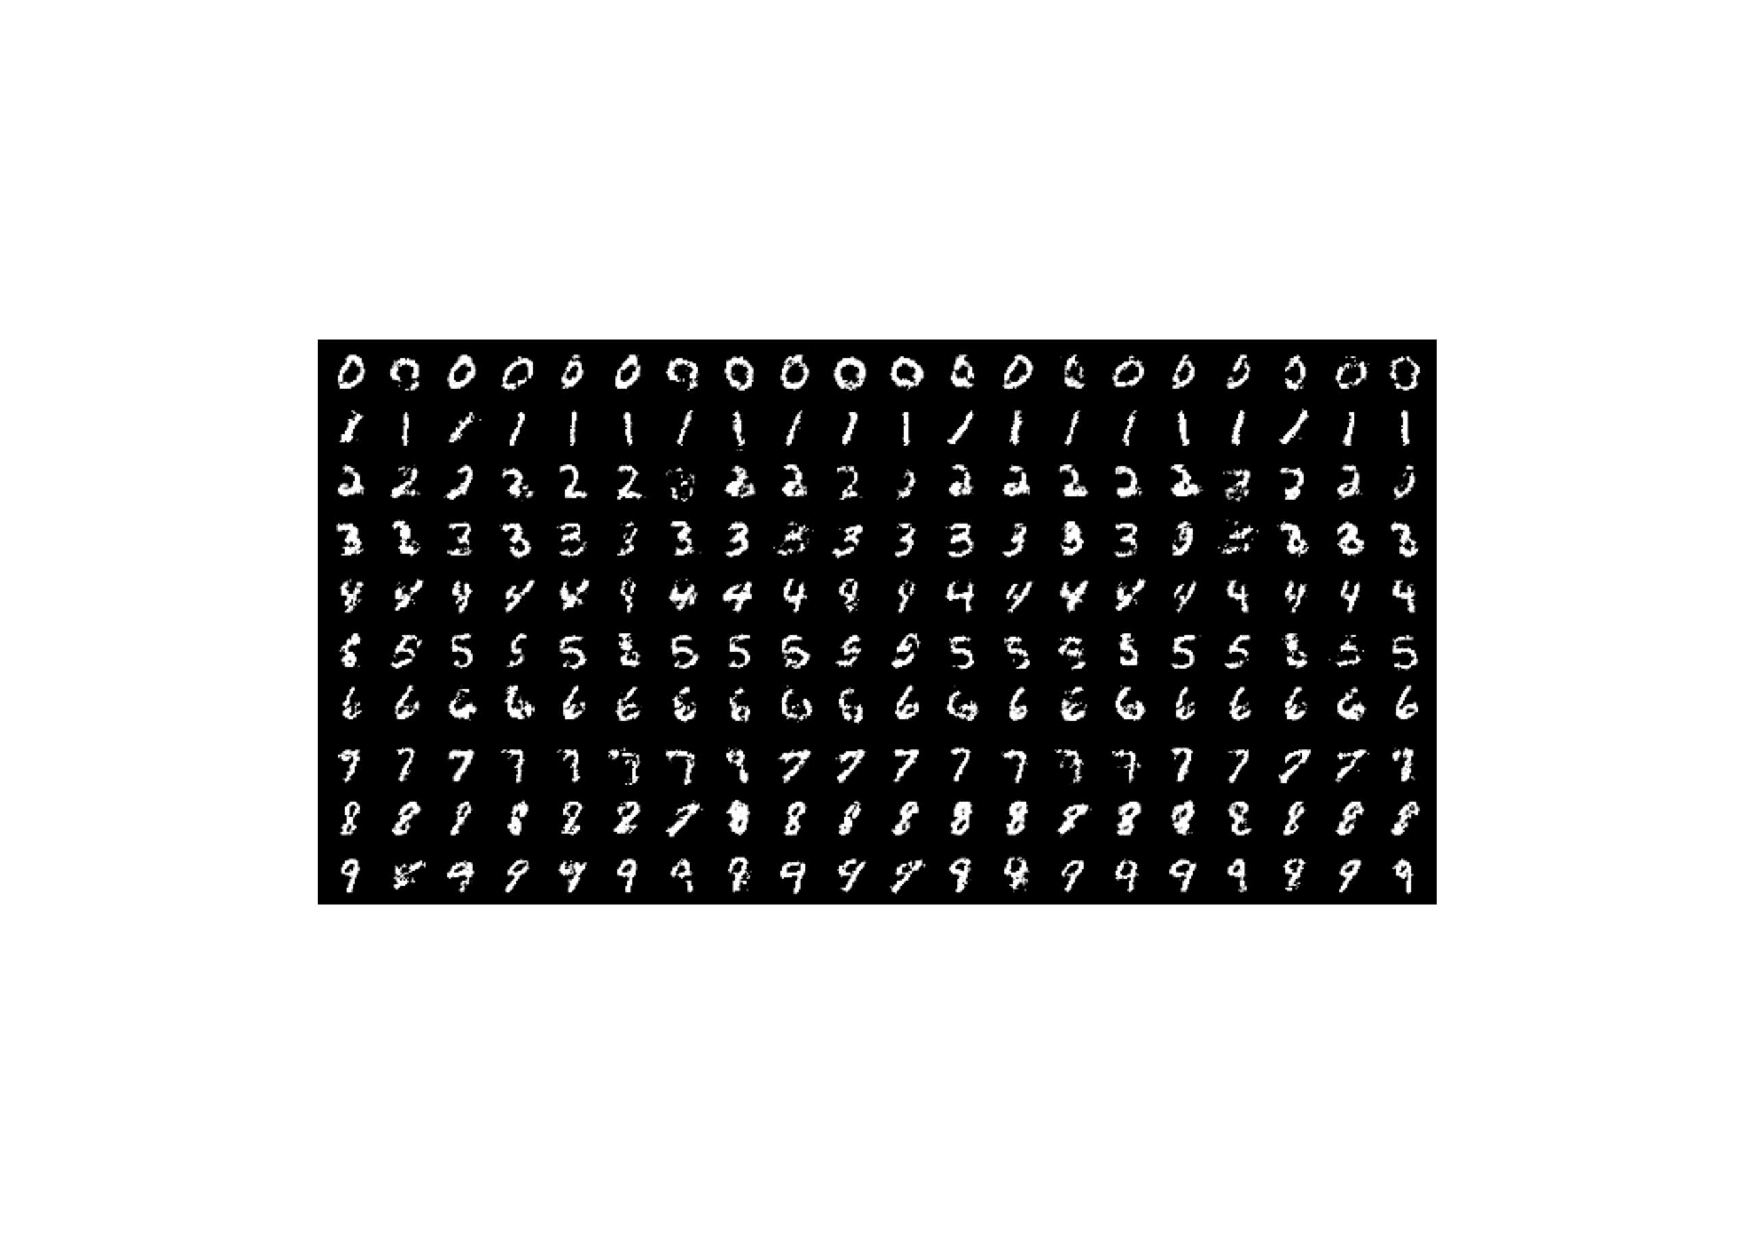
\includegraphics[width=0.5\textwidth]{figures/CGAN-result.pdf}
    \caption{cGANs指定生成手写数字}
    \label{CGAN-result}
\end{figure}

无论是GANs还是cGANs,此时仍受图像生成质量不高导致的实用价值不高的困扰。随着深度学习的发展,Alec Radford等人在2016年提出了使用卷积神经网络替换GANs中的多层感知机~\cite{DCGAN},大大提升了生成图像的质量。由于GANs这个缩写已经广泛作为生成式对抗网络的概念使用,下文将称Goodfellow等人提出的GANs模型为原始GANs。如图~\ref{fig:GAN-DCGAN}所示,原始GANs生成的人像、自然图像质量都较差;而DCGAN能够生成较高质量的卧室图片。

\begin{figure}
    \centering
    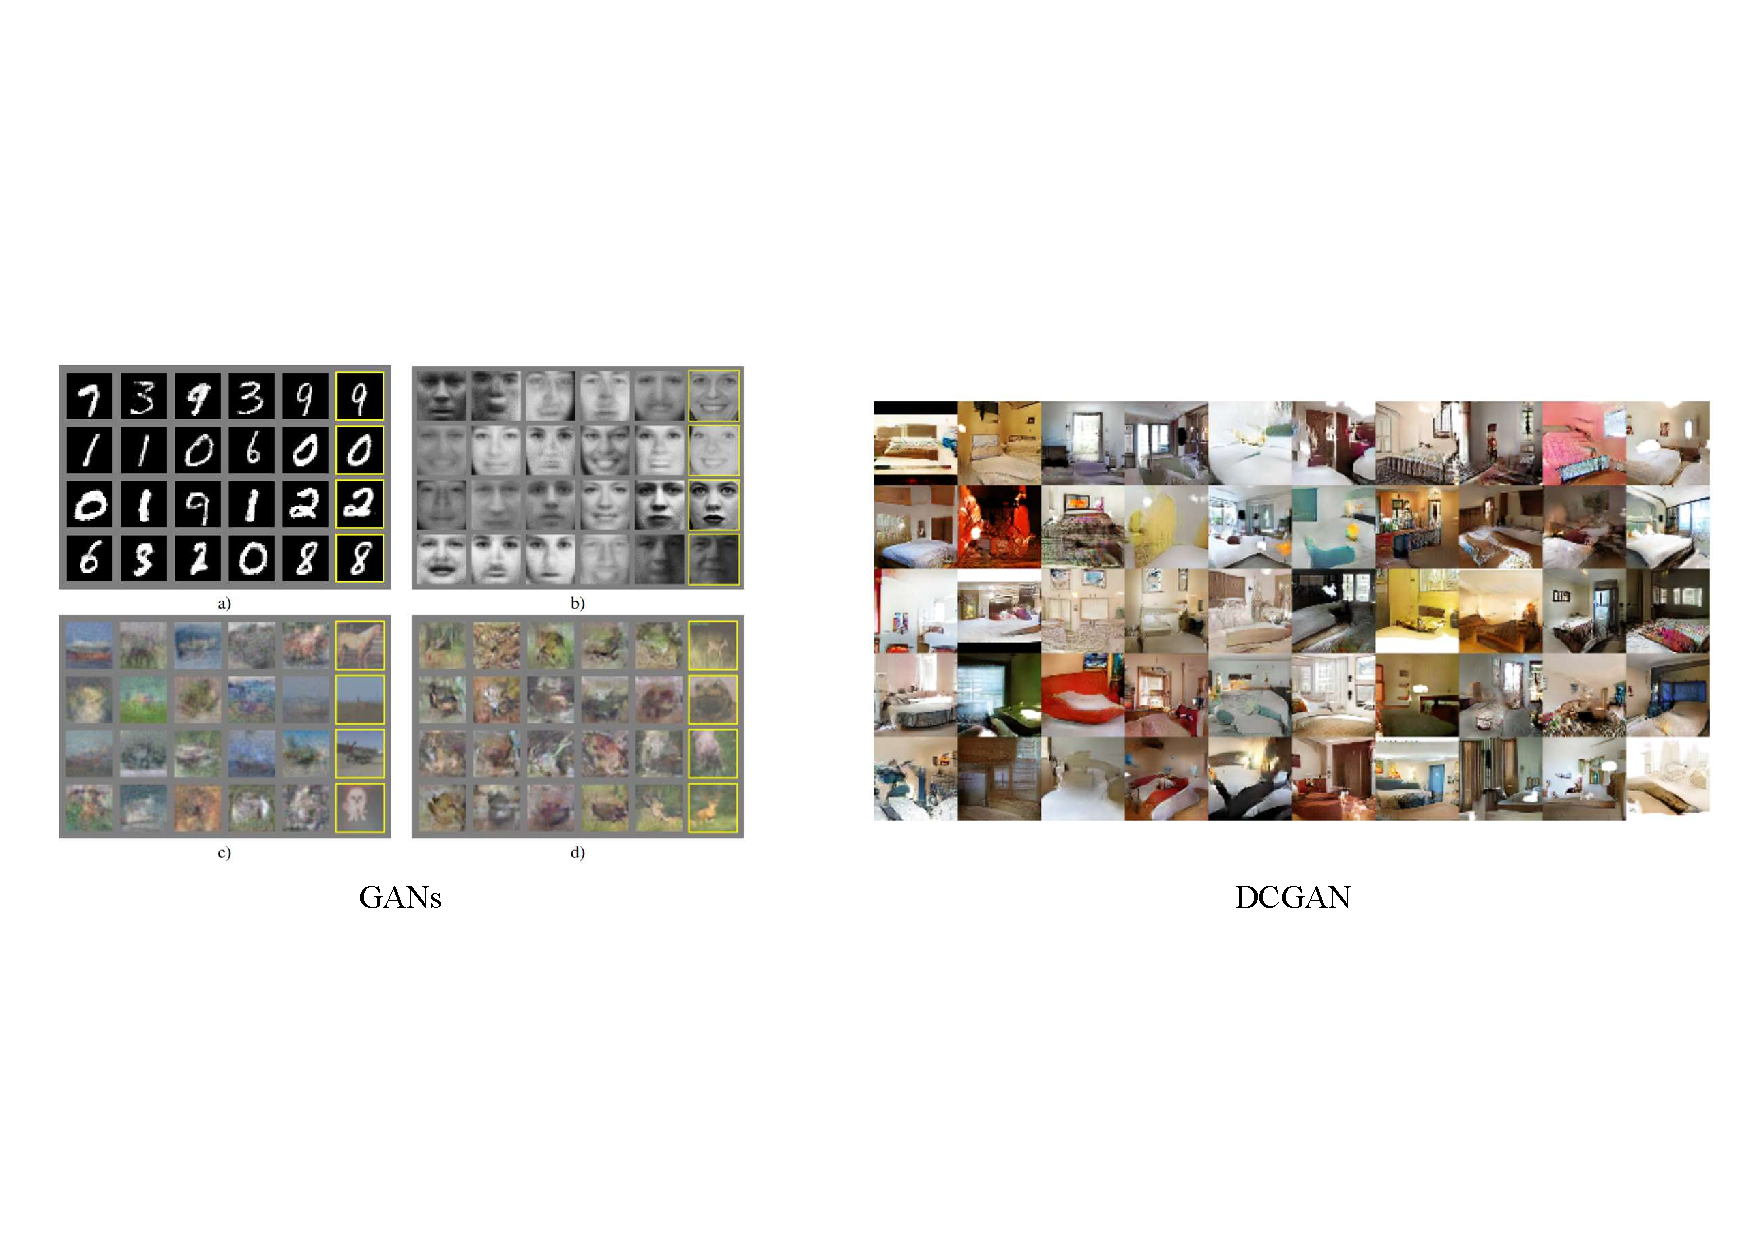
\includegraphics[width=0.8\textwidth]{figures/GAN-DCGAN.pdf}
    \caption{GANs和DCGAN的生成效果对比}
    \label{fig:GAN-DCGAN}
\end{figure}

至此,生成式对抗网络完成了它的萌芽阶段,其框架已经确定,即便是学界最新提出的GANs模型,也基本都在这一框架内:

\begin{itemize}
\item GANs由生成器和判别器两个网络组成。
\item 训练采用对抗训练的方式。判别器致力于区分生成图像与真实图像,生成器目标是生成可以“骗过”判别器的逼真图像。
\item 按照输入是否包含标签,生成式对抗网络分为非条件生成式对抗网络和条件生成式对抗网络。
\item 就图像生成而言,生成器和判别器一般由卷积神经网络实现。
\end{itemize}

\subsection{发展:迈向以假乱真的真实图像和实际应用}
由于高分辨率图像包含更多细节,判别器更容易将生成的图像与真实图像区分开来,因此在高分辨率下训练GANs是一件很困难的事。除此之外,由于显存的限制,我们在高分辨率下只能使用较小的批大小(batch size),这进一步损害了训练时的稳定性。Odena等人在2017年提出PGGAN(Progressive Growing OF GANs)~\cite{PGGAN},作者认为可以从更简单的低分辨率图像开始,随着训练的进度,逐步增大生成器和判别器的分别率。这种渐进式的训练方式大大加快了训练速度,并提高了高分辨率下的稳定性。

时间来到2019年,BigGANs~\cite{BigGANs}探索了cGANs如何通过训练更大的模型提高生成图像的质量,StyleGAN~\cite{stylegan}则展示了GANs如何生成风格各异的图像。BigGANs和StyleGAN的生成结果分别如图~\ref{fig:BigGAN}和图~\ref{fig:StyleGAN}所示。
图~\ref{fig:StyleGAN}最上面一行与最左边一列是StyleGAN生成的不同风格的人像,中间则是两种风格混合后生成的人像。作者将这种风格混合生成人像的功能称为style mixing。
可以看到无论是GANs(StyleGAN)还是cGANs(BigGANs),生成图像的质量都非常高,甚至可以说达到了“以假乱真”的程度。

\begin{figure}
    \centering
    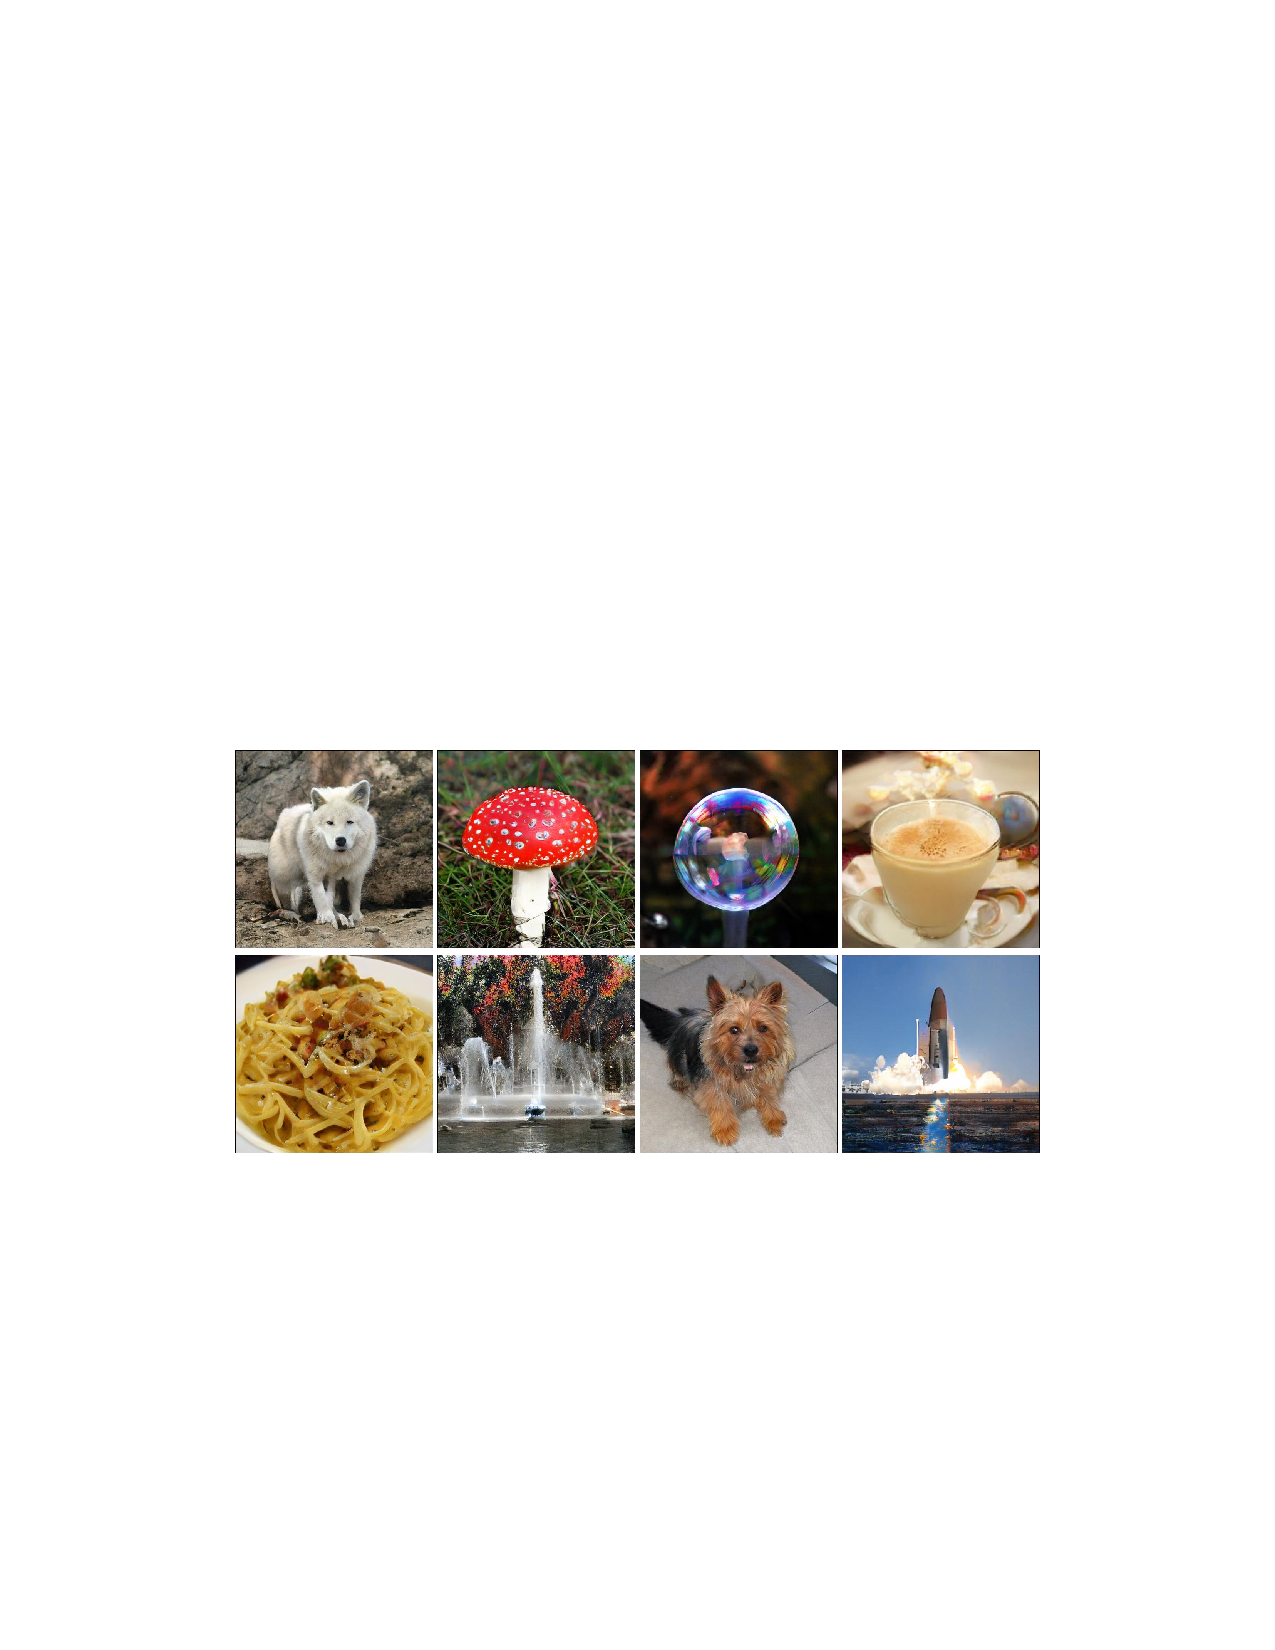
\includegraphics[width=0.6\textwidth]{figures/BigGAN.pdf}
    \caption{BigGANs的512x512分辨率下的生成图像}
    % 可以看到生成的图像种类丰富且非常真实,但放大后仍可看出些许涂抹感。
    \label{fig:BigGAN}
\end{figure}

\begin{figure}
    \centering
    \includegraphics[width=0.6\textwidth]{figures/StyleGAN.pdf}
    \caption{StyleGAN的生成结果}
    \label{fig:StyleGAN}
\end{figure}


\subsection{最新进展和应用}

正如我们在上一节提到的,我们已经能够使用GANs生成足够真实且风格迥异的图片,因此研究热点逐渐转为GANs的应用。我们在这里主要介绍两类应用,一是基于GANs的图像编辑,二是基于GANs的图像转换。

cGANs的出现,使我们能够控制生成图像的类别,但我们仍无法控制生成图像的属性。例如,我们可以使用cGANs生成年轻人和老年人两类图像,但无法具体控制人物年轻或年老的程度。实际上早在DCGAN中,作者就发现了隐空间(生成器输入又称为隐变量,输入所在的空间又称为隐空间)中的向量运算可以控制生成图像的属性。受此启发,近些年出现了非常多通过在隐空间搜索语义方向的方式实现生成图像属性编辑的工作\cite{icml2020, harkonen2020ganspace, iclr2021, interfacegan, steer,variation},我们将这类通过隐空间中向量运算改变生成图像属性的方法统称为隐空间编辑(latent-space editing)。

GANs很早就被用于图片转换(image translation,又称图像翻译),即将原域的图片转换为目标域的图片,经典的模型有Pix2Pix~\cite{pix2pix}、CycleGAN~\cite{cyclegan}等。本质上,这类用于图片转换的GANs是一种特殊的cGANs,此时原域的图片作为标签输入生成器。最近,研究人员提出CollaGAN~\cite{collagan}和Auto-GAN~\cite{AutoGAN},开始将GANs应用于多模态图像转换,一定程度上解决了多模态图像缺失的问题。


\section{问题和挑战}

据我们所知,现有的隐空间编辑多是:1.在预训练的GANs上搜索隐空间中属性对应的语义方向;2.在对应的语义方向上对隐变量进行向量运算。这类方法在做图像编辑时存在语义耦合的问题,即在改变某一属性时,其他属性也发生了变化。

在多模态图像变换方面,现有的基于GANs的方法没有充分利用模态间的一致性与互补性,这导致生成的目标模态图像出现信息损失。多模态数据广泛存在临床诊断等领域,缺失的信息可能会影响医生的决策。

\section{本文的贡献}

本文全面分析了GANs在图像编辑和多模态图像转换上遇到的问题和挑战,提供相应的解决方法:

(1)为了解决隐空间图像编辑语义耦合的问题,我们提出属性一致性网络。将输入隐变量分解为内容变量和属性变量,其中属性变量位于预定义的正交属性空间中,从而保证了图像编辑时的语义解耦。

(2)针对现有的基于GANs的多模态图像变换方法没有充分利用模态间的一致性与互补性的问题,我们提出联合注意力机制,在模型训练期间充分挖掘模态间的一致性与互补性,显著提高了多模态图像转换的质量与准确性。

\section{本文组织结构}

本文主要关注GANs在图像编辑和多模态图像转换上遇到的问题和挑战,提供相应的解决方案,并通过大量实验进行了验证,具体组织结构如下:

第一章简要梳理了生成对抗网络的发展历史,并引出了本文所关注的两个任务:图像编辑和多模态图像转换。最后总结了本文的创新点和贡献;

第二章全面介绍了生成对抗网络的原理与应用,特别是其在图像编辑和多模态图像上存在的不足;

第三章介绍了如何通过属性一致性约束,实现能够天然控制属性连续变化的生成式对抗网络,解决隐空间图像编辑中的语义耦合问题;

第四章介绍了如何使用注意力机制充分挖掘模态间的一致性与互补性,从而提高基于生成式对抗网络的多模态图像转换的质量;

第六章对全文进行总结,重点是本文的贡献和不足,为日后生成式对抗网络的研究提供了参考方向。